\documentclass[11pt]{beamer}
\usefonttheme[onlymath]{serif}

\setbeamersize{text margin left=1.5em}
\setbeamersize{text margin right=1.5em}

\setbeamertemplate{frametitle}{%
  \vskip1ex
  \usebeamerfont{frametitle}%
  \insertframetitle\par
  \vskip1ex
  \hrule
}

\setbeamertemplate{blocks}[rounded][shadow=true]

\setbeamertemplate{itemize item}{\usebeamerfont{itemize item}\textbullet}
\setbeamertemplate{itemize subitem}{\usebeamerfont{itemize subitem}\textbullet}
\setbeamertemplate{itemize subsubitem}{\usebeamerfont{itemize subsubitem}\textbullet}

\makeatletter
\geometry{%
  papersize={\fpeval{\beamer@paperwidth*1.5}pt,\fpeval{\beamer@paperheight*1.5}pt},
  hmargin=\fpeval{0.5 * 1.5}cm,% 1cm
  vmargin=0cm,%
  head=\fpeval{0.5*1.5}cm,% 0.5cm
  headsep=0pt,%
  foot=\fpeval{0.5*1.5}cm% 0.5cm
}
\makeatother

\usepackage{graphicx}
\usepackage{amsmath}
\usepackage{amssymb}
\usepackage{mathtools}

% Your custom commands (kept as is)
\newcommand{\mrm}[1]{\mathrm{#1}}
\newcommand{\mbb}[1]{\mathbb{#1}}
\newcommand{\mb}[1]{\mathbf{#1}}
\newcommand{\mc}[1]{\mathcal{#1}}
\newcommand{\tb}[1]{\textbf{#1}}

% Title, Author, etc.
\title{Stabilizing Off-Policy Q-Learning via Bootstrapping Error Reduction (BEAR)}
\author{Gwanwoo Choi} % Or keep "Gwanwoo Choi" if you prefer
\institute{MLIC}
% \date{} % To use the current date

\begin{document}

% --- Title Frame ---
\begin{frame}
    \titlepage
\end{frame}

% % --- Outline Frame ---
% \begin{frame}{Outline}
%     \tableofcontents
% \end{frame}

% % =======================================================
% \section{Introduction: The Challenge of Offline RL}
% % =======================================================

% \begin{frame}{What is Offline Reinforcement Learning?}
%     \begin{block}{Definition}
%         A paradigm in RL where an agent learns a policy from a fixed, static dataset ($\mc{D}$) without any further online interaction with the environment. Also known as Batch RL.
%     \end{block}
    
%     \begin{itemize}
%         \item Essential for domains where online interaction is impossible, expensive, or dangerous.
%         \item Examples: Healthcare, robotics, autonomous driving, recommendation systems.
%     \end{itemize}
    
%     \begin{block}{The Core Challenge}
%         How to handle the \tb{distributional shift} between the data-collecting policy and the learned policy?
%     \end{block}
% \end{frame}

% \begin{frame}{Problem 1: Distributional Shift}
%     \begin{itemize}
%         \item The dataset $\mc{D}$ was collected by a specific behavior policy ($\beta$).
%         \item The learned policy ($\pi$) attempts to improve upon $\beta$, so its action distribution will differ.
%         \item When policy $\pi$ queries the value of a state-action pair not well-represented in the data (Out-of-Distribution, OOD), the Q-function must extrapolate, leading to inaccurate value estimates.
%     \end{itemize}
    
%     \begin{block}{Extrapolation Error}
%         Q-function estimates for OOD state-action pairs are unreliable and can contain large errors.
%     \end{block}
% \end{frame}

% \begin{frame}{Problem 2: Bootstrapping Error Accumulation}
%     \begin{itemize}
%         \item The Bellman update bootstraps, using previous Q-estimates to update the current Q-function.
%         \[ Q_k(s,a) \approx r + \gamma \max_{a'} Q_{k-1}(s', a') \]
%         \item If the $\max_{a'}$ operator selects an OOD action, the erroneous $Q_{k-1}(s', a')$ value becomes the target.
%         \item This error is then propagated to other state-action pairs through subsequent updates.
%         \item Eventually, the entire Q-function can become corrupted, leading to learning failure.
%     \end{itemize}
%     \begin{center}
%         \tb{This is the fundamental reason why naive off-policy RL (e.g., TD3) fails on static offline datasets.}
%     \end{center}
% \end{frame}


% \begin{frame}{Theoretical Performance Bound (Theorem 4.1)}
%     \begin{block}{Suboptimality Bound}
%         This theorem formalizes the trade-off by bounding the suboptimality of the learned value function. The bound is given by:
%         \[
%         \lim_{k \to \infty} \mbb{E}_{\rho_0}[|V^{\pi_k}(s) - V^*(s)|] \le \frac{\gamma}{(1-\gamma)^2} \left( C(\Pi) \mbb{E}_{\mu} [\max_{\pi \in \Pi} \mbb{E}_{\pi}[\delta(s,a)]] + \frac{1-\gamma}{\gamma} \alpha(\Pi) \right)
%         \]
%     \end{block}
    
%     \begin{itemize}
%         \item The left side, $|V^{\pi_k}(s) - V^*(s)|$, represents the \tb{suboptimality gap} of the learned policy.
%         \item The total error is amplified by the \tb{Concentrability Coefficient ($C(\Pi)$)}, which measures distributional shift.
%         \item The other error sources are the \tb{Bellman Error ($\delta$)} from function approximation and the \tb{Suboptimality Constant ($\alpha(\Pi)$)} from the limited policy set.
%     \end{itemize}

%     \begin{center}
%         \tb{To minimize this bound, we must balance keeping $C(\Pi)$ small (staying on-support) with keeping $\alpha(\Pi)$ small (allowing policy improvement).}
%     \end{center}
% \end{frame}

% \begin{frame}{Key Concepts: $C(\Pi)$ and $\alpha(\Pi)$}
%     To analyze this problem, we define two important constants.

%     \begin{block}{1. Concentrability Coefficient: $C(\Pi)$}
%         Measures how much the state visitation distribution of a policy set $\Pi$ deviates from the data distribution $\mu$.
%         \begin{itemize}
%             \item Represents the \tb{amplification of error} due to distributional shift.
%             \item As $\Pi$ deviates from the data distribution, $C(\Pi)$ increases (minimum value is 1).
%         \end{itemize}
%     \end{block}

%     \begin{block}{2. Suboptimality Constant: $\alpha(\Pi)$}
%         Measures how far the best policy within the set $\Pi$ is from the true optimal policy.
%         \begin{itemize}
%             \item Represents the \tb{inherent limitation} of the policy set's expressiveness.
%             \item As $\Pi$ includes more diverse and better policies, $\alpha(\Pi)$ decreases.
%         \end{itemize}
%     \end{block}
% \end{frame}


\begin{frame}{Sources of Suboptimality in Offline RL}
    When learning from a fixed dataset, two primary sources of error can lead to a suboptimal final policy.

    \begin{block}{1. Suboptimality Bias}
        The set of candidate policies, $\Pi$, that the algorithm considers might be too restrictive.
        \begin{itemize}
            \item If the true optimal policy, $\pi^*$, is not contained within $\Pi$, the best policy we can possibly find is inherently suboptimal from the start.
            \item This error arises from the \tb{limited expressiveness} of the policy set.
        \end{itemize}
    \end{block}

    \begin{block}{2. Distributional Shift}
        The policies used for Bellman backups (derived from $\Pi$) can differ significantly from the data-collection policy, $\beta$.
        \begin{itemize}
            \item This mismatch leads to querying the values of Out-of-Distribution (OOD) actions.
            \item This results in \tb{extrapolation errors} which are then amplified through the bootstrapping process, as seen in Figure 2.
        \end{itemize}
    \end{block}
\end{frame}


\begin{frame}{Formalizing the Error Components: $\alpha(\Pi)$ and $C(\Pi)$}
    We can quantify these two error sources with the following definitions.

    \begin{block}{Suboptimality Constant: $\alpha(\Pi)$}
        This measures the suboptimality bias.
        \[ \alpha(\Pi) = \max_{s,a} |T^\Pi Q^*(s,a) - TQ^*(s,a)| \]
        \begin{itemize}
            \item It captures the maximum difference between the standard Bellman operator ($TQ^*$) and an operator constrained to policies in $\Pi$ ($T^\Pi Q^*$).
            \item A \tb{larger, more expressive $\Pi$} leads to a \tb{smaller $\alpha(\Pi)$}.
        \end{itemize}
    \end{block}

    \begin{block}{Concentrability Coefficient: $C(\Pi)$}
        This measures the effect of distributional shift, based on the assumption:
        \[ \rho_0 P^{\pi_1} \dots P^{\pi_k}(s) \le c(k) \mu(s) \]
        \begin{itemize}
            \item It bounds the ratio between the state distribution generated by policies in $\Pi$ and the dataset's state distribution $\mu$.
            \item $C(\Pi)$ is a weighted sum of these mismatch coefficients, $c(k)$. A \tb{larger, more diverse $\Pi$} can lead to a \tb{larger $C(\Pi)$}.
        \end{itemize}
    \end{block}
\end{frame}


\begin{frame}{The Overall Performance Bound (Theorem 4.1)}
    This theorem combines both error sources to provide an upper bound on the final policy's suboptimality.

    \begin{block}{The Suboptimality Bound}
        \[
        \lim_{k \to \infty} \mbb{E}_{\rho_0}[|V^{\pi_k}(s) - V^*(s)|] \le \frac{\gamma}{(1-\gamma)^2} \left( C(\Pi) \mbb{E}_{\mu} [\dots] + \frac{1-\gamma}{\gamma} \alpha(\Pi) \right)
        \]
    \end{block}
    
    \begin{itemize}
        \item The \tb{left-hand side} is the final suboptimality gap we want to minimize.
        \item The \tb{right-hand side} shows that the total error depends on two key terms.
        \item \tb{Observation 1}: The distributional shift error, $C(\Pi)$, acts as a \tb{multiplier} on the Bellman error term. A large $C(\Pi)$ can amplify even small approximation errors.
        \item \tb{Observation 2}: The bound is a sum of the $C(\Pi)$-weighted term and the $\alpha(\Pi)$ term. This mathematically formalizes the trade-off.
    \end{itemize}

    \begin{center}
        \tb{To guarantee good performance, an algorithm must balance keeping $C(\Pi)$ small with keeping $\alpha(\Pi)$ small.}
    \end{center}
\end{frame}

\begin{frame}{The Core Dilemma: $C(\Pi)$ vs. $\alpha(\Pi)$ Trade-off}
    The performance of an offline RL algorithm depends on balancing these two sources of error.

    \begin{columns}[T]
        \begin{column}{.5\textwidth}
            \begin{block}{Shrinking the policy set $\Pi$}
                (e.g., similar to behavior policy)
                \begin{itemize}
                    \item $C(\Pi) \downarrow$ (Safety $\uparrow$)
                    \item $\alpha(\Pi) \uparrow$ (Optimality $\downarrow$)
                \end{itemize}
            \end{block}
        \end{column}
        \begin{column}{.5\textwidth}
            \begin{block}{Expanding the policy set $\Pi$}
                (e.g., considering all policies)
                \begin{itemize}
                    \item $C(\Pi) \uparrow$ (Safety $\downarrow$)
                    \item $\alpha(\Pi) \downarrow$ (Optimality $\uparrow$)
                \end{itemize}
            \end{block}
        \end{column}
    \end{columns}

    \vspace{1cm}
    \begin{center}
        \tb{Goal: Find an optimal policy set $\Pi$ that minimizes $\alpha(\Pi)$ while keeping $C(\Pi)$ bounded.}
    \end{center}
\end{frame}


\begin{frame}{Visualizing the Core Problem: Error Propagation (Fig. 2)}
    \begin{columns}[T] % Divide the frame into columns
        
        % Left Column for the Figure
        \begin{column}{0.5\textwidth}
            \begin{figure}
                \centering
                % --- Please insert Figure 2 from the BEAR paper here ---
                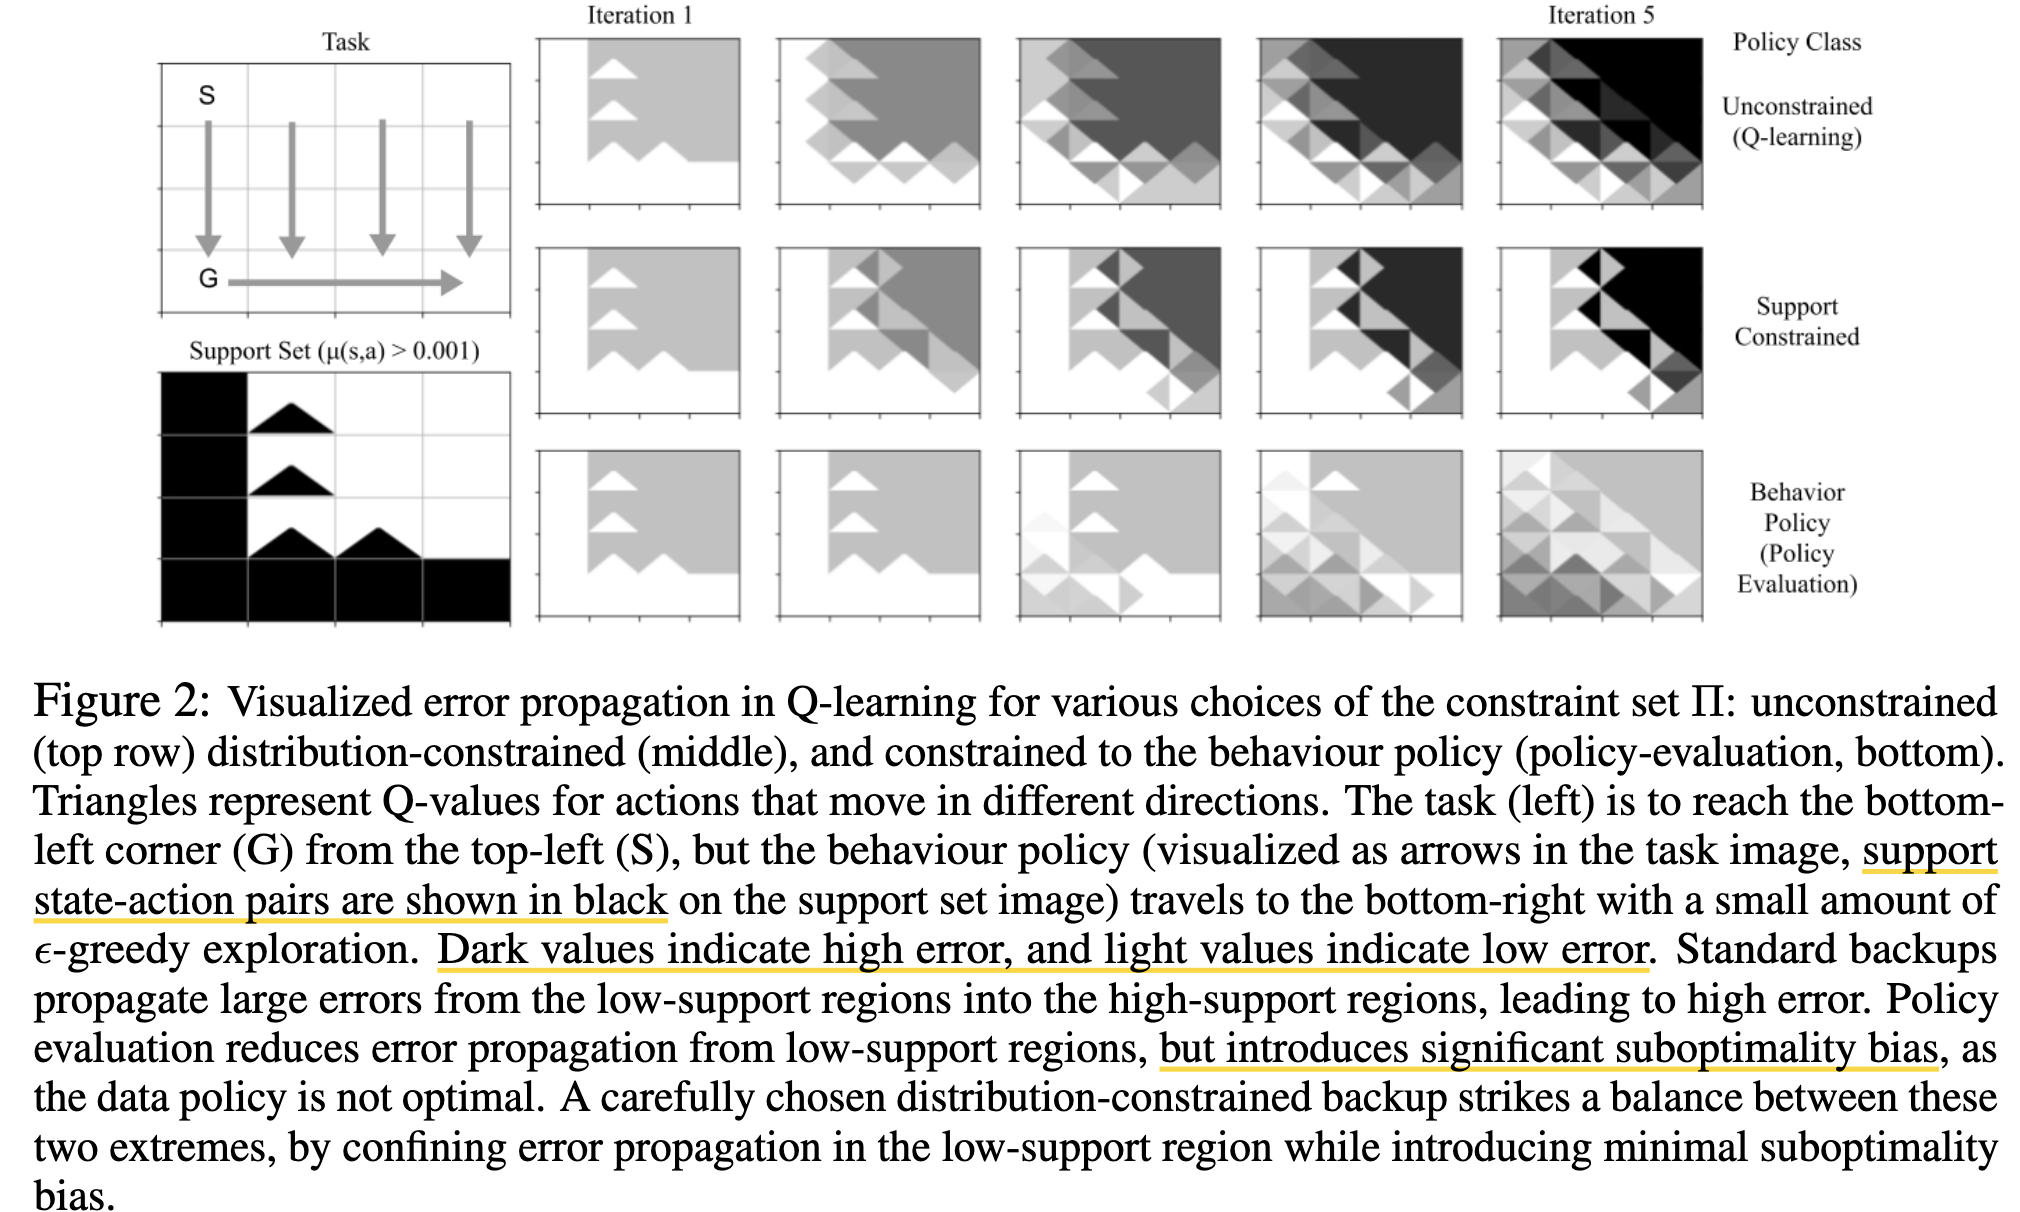
\includegraphics[width=\textwidth]{Figure2.png}
                \caption{Error propagation in a gridworld.}
            \end{figure}
        \end{column}
        
        % Right Column for the Explanation
        \begin{column}{0.5\textwidth}
            \begin{itemize}
                \item \tb{Setup}: The data is collected by a policy moving away from the optimal goal, creating an Out-of-Distribution (OOD) region with high initial error (top-right).
                \vspace{1em}
                \item \tb{Unconstrained (Q-learning)}: Fails. The $\max$ operator propagates high error from the OOD region into the data-supported region, corrupting the Q-values.
                \vspace{1em}
                \item \tb{Behavior Policy (Policy Eval.)}: Stable but suboptimal. It avoids error propagation but cannot learn a better policy.
                \vspace{1em}
                \item \tb{Support Constrained (BEAR's idea)}: Succeeds. It strikes a balance by confining error propagation to the OOD region while allowing for stable policy improvement.
            \end{itemize}
        \end{column}
        
    \end{columns}
\end{frame}

\begin{frame}{BEAR: Core Idea and Components}
    \begin{block}{Core Idea}
        Explicitly constrain the learned policy to lie within the \tb{support} of the behavior policy's data distribution.
        \begin{itemize}
            \item "Search for the optimal policy only within the realm of actions the data has shown us."
            \item This prevents $C(\Pi)$ from exploding, thus avoiding error accumulation.
        \end{itemize}
    \end{block}

    \begin{block}{Key Components}
        \begin{enumerate}
            \item \tb{Ensemble of Q-functions}: Learn multiple Q-functions and use the minimum value for conservative estimation, enhancing stability.
            \item \tb{MMD-based Support Constraint}: Since the behavior policy $\beta$ is unknown, use a sample-based distance metric, Maximum Mean Discrepancy (MMD), to ensure the learned policy $\pi$ stays close to $\beta$.
        \end{enumerate}
    \end{block}
\end{frame}

\begin{frame}{The MMD (Maximum Mean Discrepancy) Constraint}
    \begin{itemize}
        \item \tb{Problem}: We cannot directly use the theoretical constraint ($\pi(a|s)=0 \text{ if } \beta(a|s)<\epsilon$) because the true distribution of $\beta$ is unknown.
        \item \tb{Solution}: Use MMD, which can compute the distance between two distributions using only samples.
    \end{itemize}
    
    \begin{block}{Constrained Policy Update Objective}
    \begin{align*}
    \pi_\phi := \max_{\pi} \quad & \mbb{E}_{s \sim \mc{D}, a \sim \pi(\cdot|s)} \left[ \min_{j=1,..,K} \hat{Q}_j(s,a) \right] \\
    \text{s.t.} \quad & \mbb{E}_{s \sim \mc{D}} \left[ \text{MMD}(\mc{D}(s), \pi(\cdot|s)) \right] \leq \epsilon
    \end{align*}
    \end{block}

    \begin{itemize}
        \item \tb{Objective}: Maximize the conservative expectation of the Q-value.
        \item \tb{Constraint}: The MMD distance between the learned policy $\pi$ and the data distribution $\mc{D}$ must not exceed a threshold $\epsilon$.
    \end{itemize}
\end{frame}

% =======================================================
\section{Experimental Results and Analysis}
% =======================================================

\begin{frame}{Experiment 1: Performance on Medium-Quality Data}
    \begin{itemize}
        \item The most realistic scenario: data collected from a partially trained, imperfect policy.
        \item The magenta dashed line indicates the average performance of the data-collection policy.
    \end{itemize}
    
    \begin{figure}
        \centering
        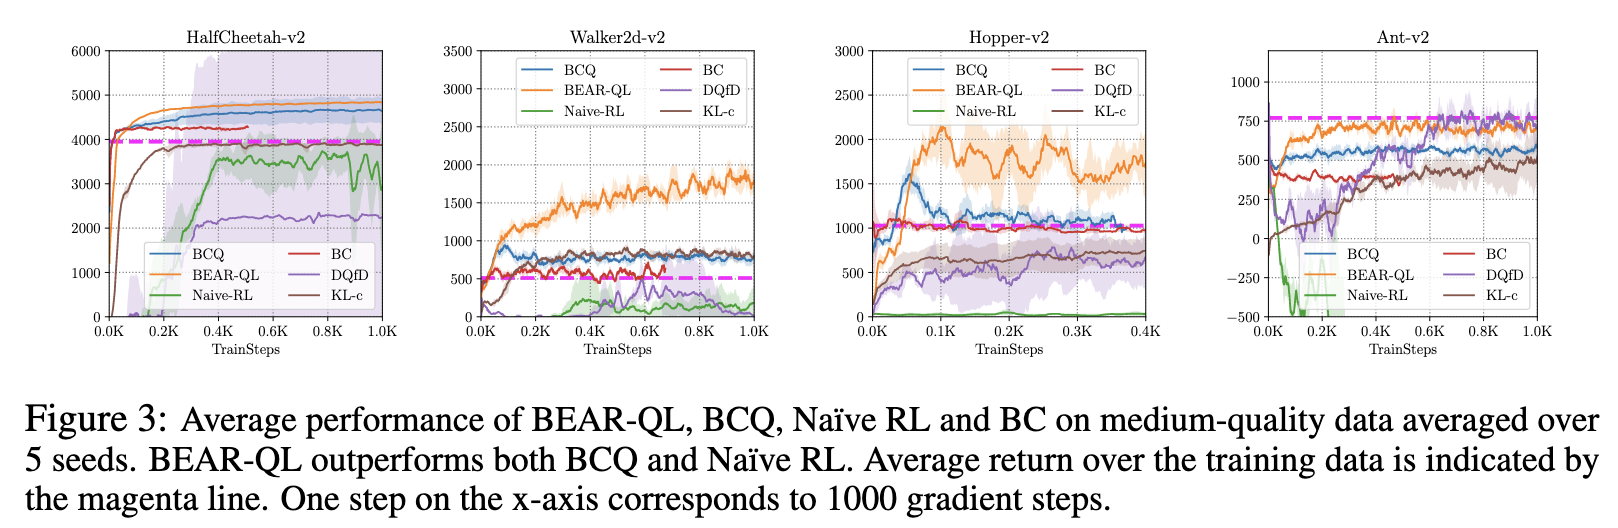
\includegraphics[width=0.9\textwidth]{Figure3.png}
        \caption{Performance on medium-quality data.}
    \end{figure}
    
    \begin{itemize}
        \item \tb{BEAR-QL} consistently outperforms baselines and successfully improves upon the behavior policy.
        \item \tb{Naive-RL} fails to learn and suffers from performance degradation due to error accumulation.
    \end{itemize}
\end{frame}

\begin{frame}{Experiment 2: Performance on Extreme Datasets}
    \begin{columns}[T]
        \begin{column}{.5\textwidth}
            \begin{block}{Random Data}
                \begin{figure}
                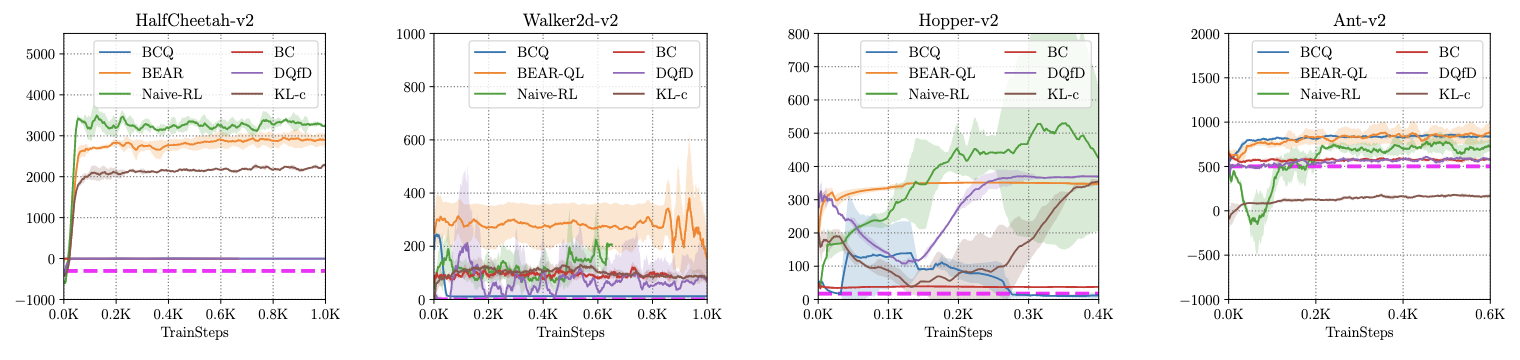
\includegraphics[width=\textwidth]{Figure5Top.png}
                \end{figure}
                \begin{itemize}
                    \item \tb{Goal}: Test policy \textit{improvement}.
                    \item \tb{BEAR}: Succeeds.
                    \item \tb{BCQ}: Fails, as it is too conservative to improve upon random behavior.
                \end{itemize}
            \end{block}
        \end{column}
        \begin{column}{.5\textwidth}
            \begin{block}{Optimal Data}
                \begin{figure}
                % --- Insert bottom row of Figure 5 ---
                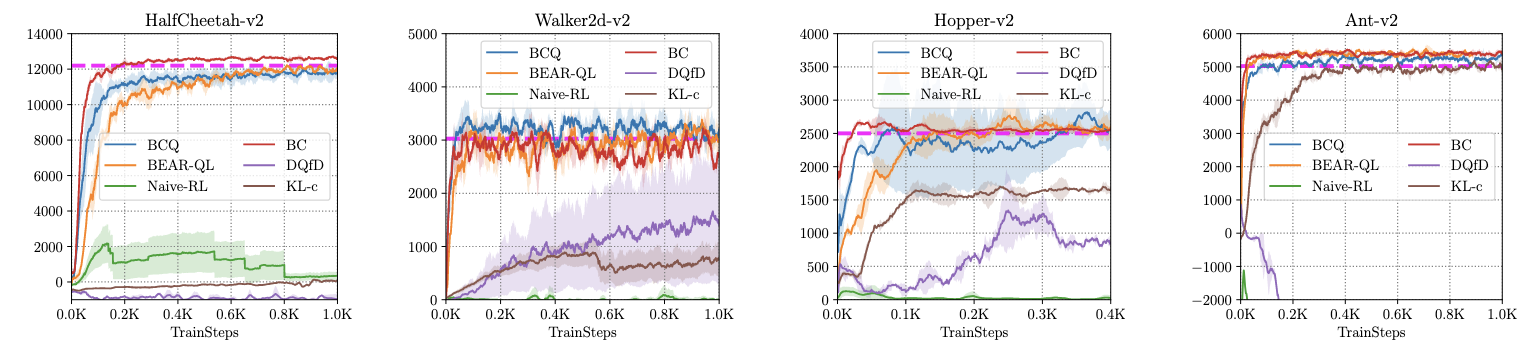
\includegraphics[width=\textwidth]{Figure5Bottom.png}
                \end{figure}
                \begin{itemize}
                    \item \tb{Goal}: Test policy \textit{stability}.
                    \item \tb{BEAR, BCQ}: Succeed.
                    \item \tb{Naive-RL}: Fails catastrophically due to OOD errors.
                \end{itemize}
            \end{block}
        \end{column}
    \end{columns}
    
    \begin{block}{Conclusion}
        BEAR is the only algorithm that demonstrates robustness across the full spectrum of data quality.
    \end{block}
\end{frame}

\begin{frame}{Ablation Studies: Validating BEAR's Design}
    \begin{columns}[T]
        \begin{column}{.5\textwidth}
            \begin{block}{MMD vs KL-Divergence}
                \begin{figure}
                 % --- Insert Figure 6a ---
                 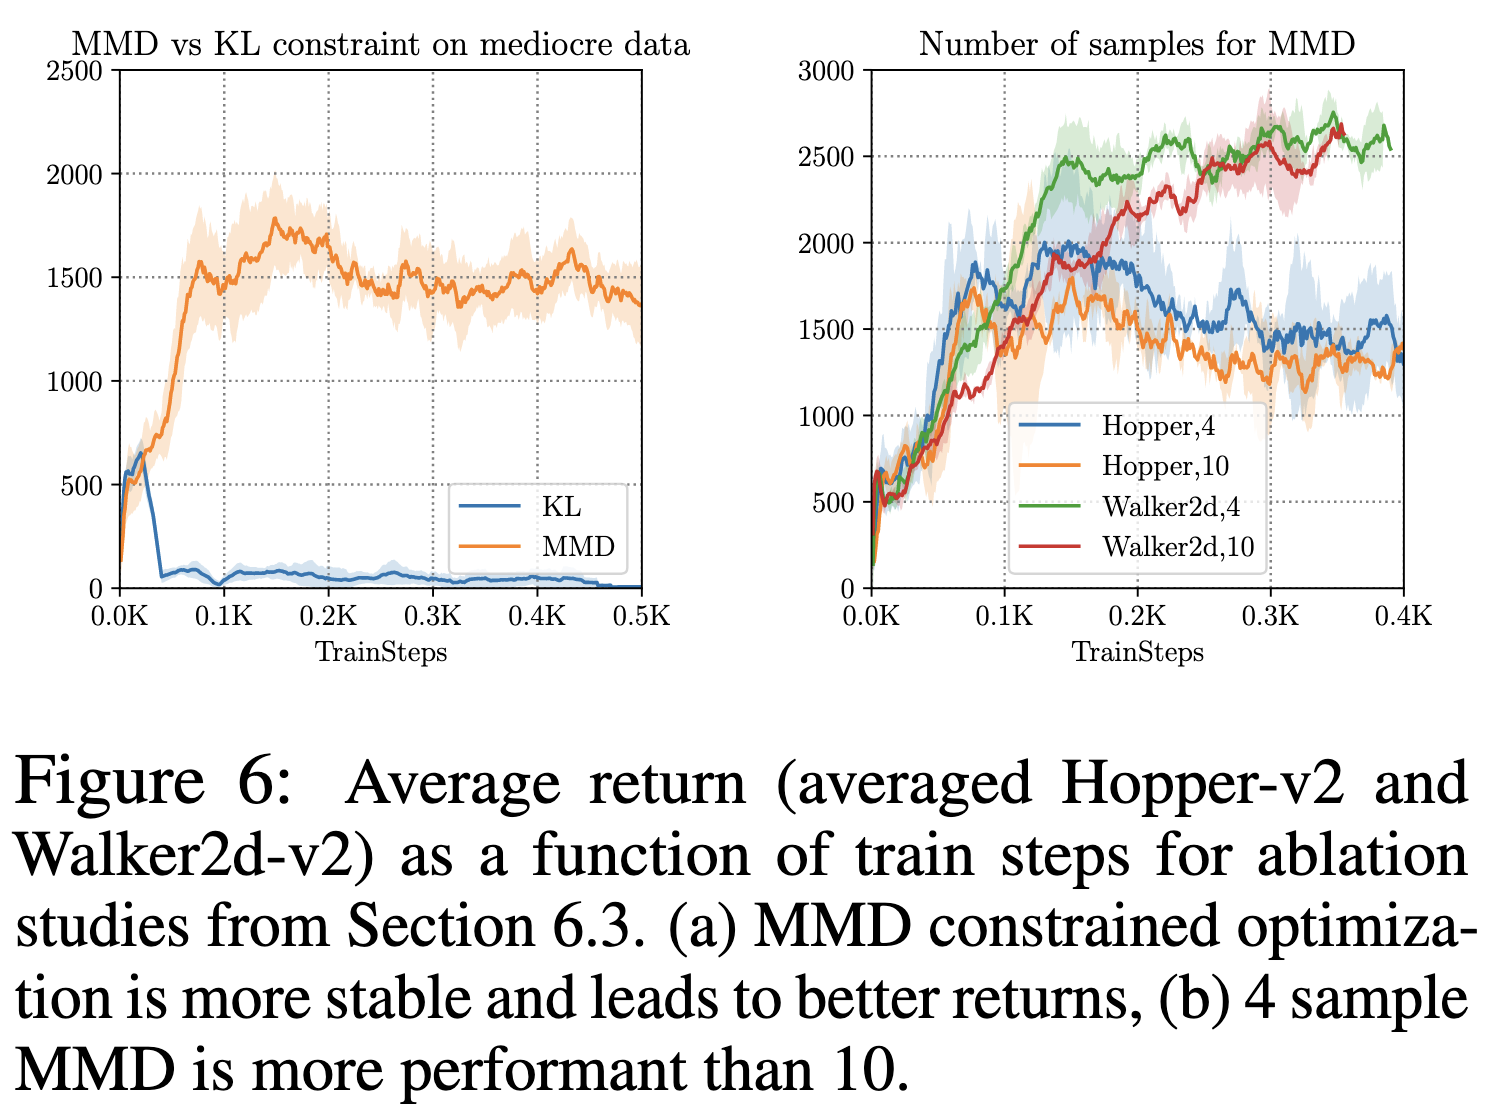
\includegraphics[width=\textwidth]{Figure6.png}
                \end{figure}
                 \begin{itemize}
                     \item \tb{Question}: Why use MMD?
                     \item \tb{Result}: The KL constraint is too strict (density matching), causing learning to fail. MMD provides a better balance (support matching).
                 \end{itemize}
            \end{block}
        \end{column}
        \begin{column}{.5\textwidth}
            \begin{block}{Number of MMD Samples}
                 \begin{figure}
                 % --- Insert Figure 6b ---
                 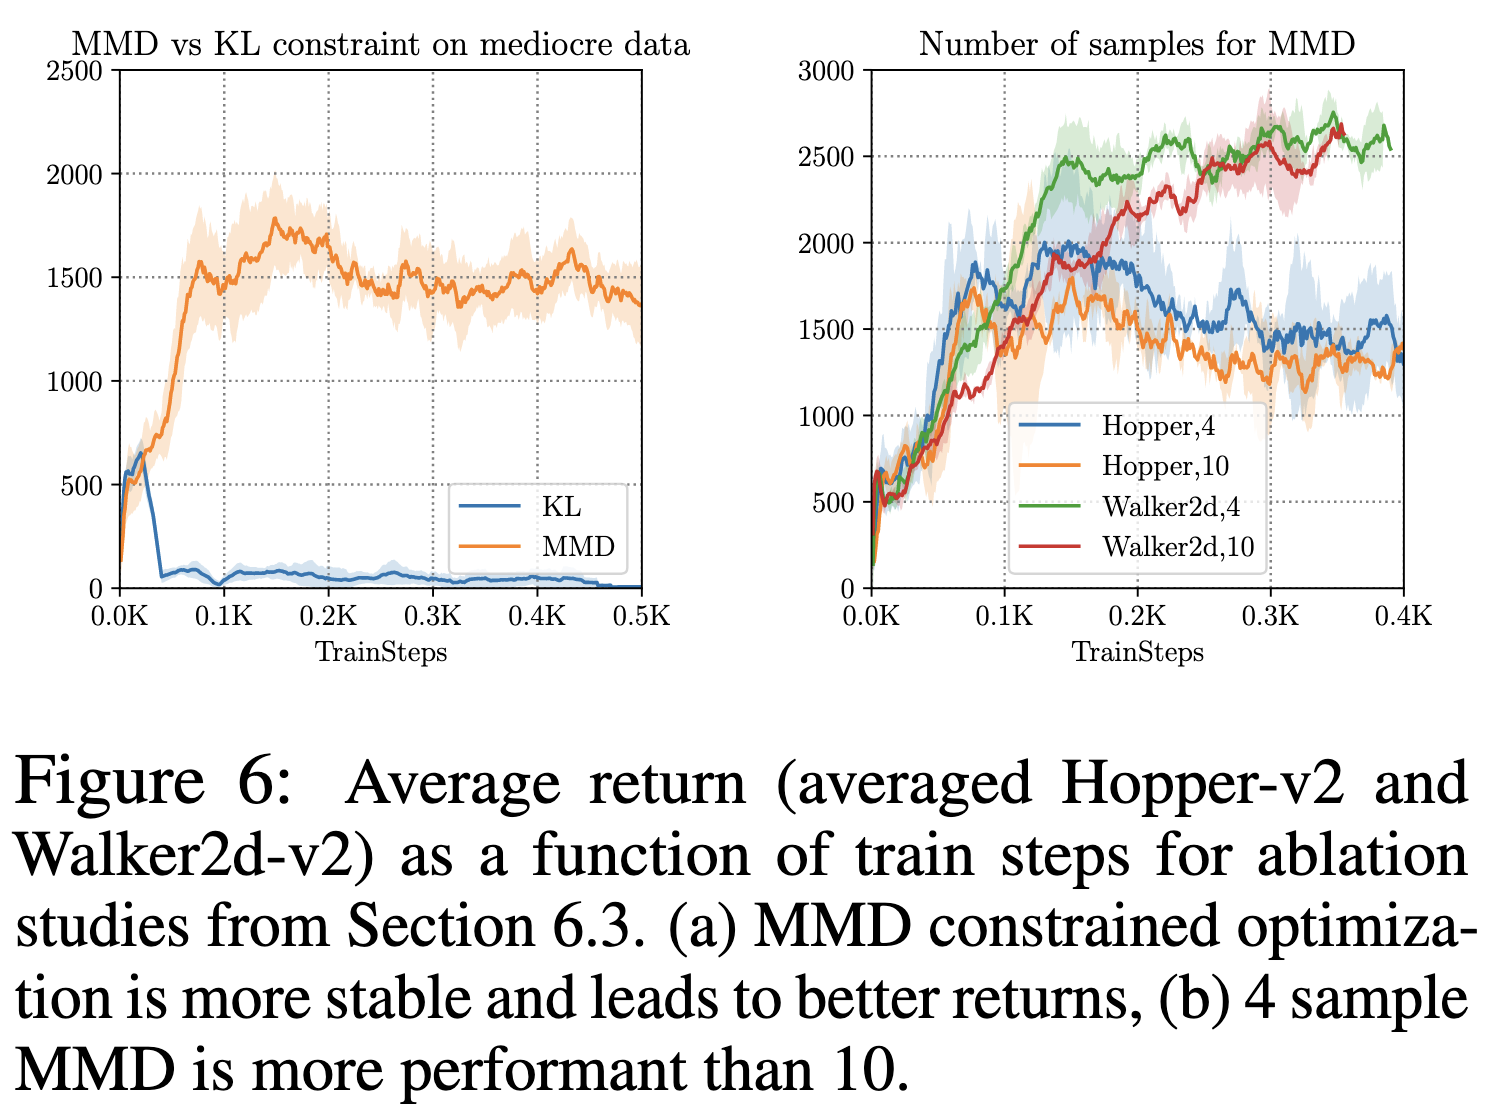
\includegraphics[width=\textwidth]{Figure6.png}
                 \end{figure}
                 \begin{itemize}
                     \item \tb{Question}: How many samples `n`?
                     \item \tb{Result}: A small number of samples (n=4) performs better, likely acting as a form of regularization.
                 \end{itemize}
            \end{block}
        \end{column}
    \end{columns}

    \begin{center}
        \tb{These studies confirm that BEAR's core design choices are crucial for its performance.}
    \end{center}
\end{frame}

% =======================================================
\section{Conclusion}
% =======================================================

% \begin{frame}{Conclusion}
%     \begin{itemize}
%         \item The key challenge in offline RL is \tb{bootstrapping error accumulation} caused by distributional shift.
%         \item This problem can be analyzed through the theoretical \tb{trade-off} between the concentrability ($C(\Pi)$) and suboptimality ($\alpha(\Pi)$) constants.
%         \item \tb{BEAR} effectively solves this by using an \tb{MMD-based constraint} to ensure the learned policy stays within the support of the data distribution.
%         \item Experiments show that BEAR achieves \tb{robust, state-of-the-art performance} across a wide variety of datasets and environments.
%     \end{itemize}
%     \begin{block}{Final Summary}
%         BEAR successfully combines theoretical insights with a practical implementation to create a robust and effective algorithm for offline reinforcement learning.
%     \end{block}
% \end{frame}


\end{document}